\begin{figure}
    \centering
    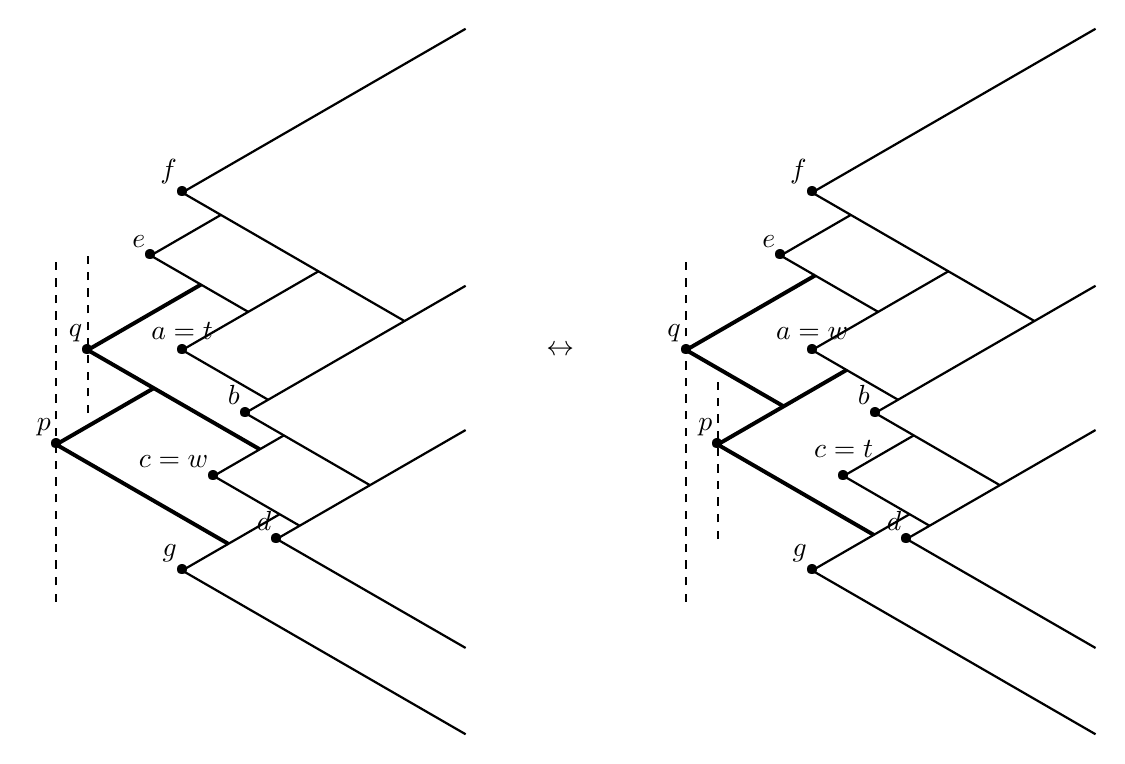
\begin{tikzpicture}[thick, scale=0.4]
        \node[label={[label distance = -3mm]160:$p$}] at
        (2.00, 2.00) {\textbullet};
        \node[label={[label distance = -3mm]160:$q$}] at
        (3.00, 5.00) {\textbullet};
        \node[label={[label distance = -2mm]90:$a = t$}] at
        (6.00, 5.00) {\textbullet};
        \node[label={[label distance = -3mm]160:$b$}] at
        (8.00, 3.00) {\textbullet};
        \node[label={[label distance = -3mm]160:$c = w$}] at
        (7.00, 1.00) {\textbullet};
        \node[label={[label distance = -3mm]160:$d$}] at
        (9.00, -1.00) {\textbullet};
        \node[label={[label distance = -3mm]160:$e$}] at
        (5.00, 8.00) {\textbullet};
        \node[label={[label distance = -3mm]160:$f$}] at
        (6.00, 10.00) {\textbullet};
        \node[label={[label distance = -3mm]160:$g$}] at
        (6.00, -2.00) {\textbullet};
        % d cone
        \draw (9.00, -1.00) -- (15.00, -4.46);
        \draw (9.00, -1.00) -- (15.00, 2.46);
        % b cone
        \draw (8.00, 3.00) -- (11.96, 0.71);
        \draw (8.00, 3.00) -- (15.00, 7.04);
        % c cone
        \draw (7.00, 1.00) -- (9.73, -0.58);
        \draw (7.00, 1.00) -- (9.23, 2.29);
        % f cone
        \draw (6.00, 10.00) -- (13.06, 5.92);
        \draw (6.00, 10.00) -- (15.00, 15.20);
        % g cone
        \draw (6.00, -2.00) -- (15.00, -7.20);
        \draw (6.00, -2.00) -- (9.10, -0.21);
        % a cone
        \draw (6.00, 5.00) -- (8.73, 3.42);
        \draw (6.00, 5.00) -- (10.33, 7.50);
        % e cone
        \draw (5.00, 8.00) -- (8.10, 6.21);
        \draw (5.00, 8.00) -- (7.23, 9.29);
        % q cone
        \draw[line width = 0.5mm] (3.00, 5.00) -- (8.46, 1.85);
        \draw[line width = 0.5mm] (3.00, 5.00) -- (6.60, 7.08);
        % p cone
        \draw[line width = 0.5mm] (2.00, 2.00) -- (7.46, -1.15);
        \draw[line width = 0.5mm] (2.00, 2.00) -- (5.10, 3.79);

        \draw[dashed] (2, -3) -- (2, 8);
        \draw[dashed] (3, 3) -- (3, 8);

        \node at (18, 5) {$ \leftrightarrow$};

        \node[label={[label distance = -3mm]160:$p$}] at
        (23.00, 2.00) {\textbullet};
        \node[label={[label distance = -3mm]160:$q$}] at
        (22.00, 5.00) {\textbullet};
        \node[label={[label distance = -2mm]90:$a = w$}] at
        (26.00, 5.00) {\textbullet};
        \node[label={[label distance = -3mm]160:$b$}] at
        (28.00, 3.00) {\textbullet};
        \node[label={[label distance = -1mm]90:$c = t$}] at
        (27.00, 1.00) {\textbullet};
        \node[label={[label distance = -3mm]160:$d$}] at
        (29.00, -1.00) {\textbullet};
        \node[label={[label distance = -3mm]160:$e$}] at
        (25.00, 8.00) {\textbullet};
        \node[label={[label distance = -3mm]160:$f$}] at
        (26.00, 10.00) {\textbullet};
        \node[label={[label distance = -3mm]160:$g$}] at
        (26.00, -2.00) {\textbullet};
        % d cone
        \draw (29.00, -1.00) -- (35.00, -4.46);
        \draw (29.00, -1.00) -- (35.00, 2.46);
        % b cone
        \draw (28.00, 3.00) -- (31.96, 0.71);
        \draw (28.00, 3.00) -- (35.00, 7.04);
        % c cone
        \draw (27.00, 1.00) -- (29.73, -0.58);
        \draw (27.00, 1.00) -- (29.23, 2.29);
        % f cone
        \draw (26.00, 10.00) -- (33.06, 5.92);
        \draw (26.00, 10.00) -- (35.00, 15.20);
        % g cone
        \draw (26.00, -2.00) -- (35.00, -7.20);
        \draw (26.00, -2.00) -- (29.10, -0.21);
        % a cone
        \draw (26.00, 5.00) -- (28.73, 3.42);
        \draw (26.00, 5.00) -- (30.33, 7.50);
        % e cone
        \draw (25.00, 8.00) -- (28.10, 6.21);
        \draw (25.00, 8.00) -- (27.23, 9.29);
        % p cone
        \draw[line width = 0.5mm] (23.00, 2.00) -- (27.96, -0.87);
        \draw[line width = 0.5mm] (23.00, 2.00) -- (27.10, 4.37);
        % q cone
        \draw[line width = 0.5mm] (22.00, 5.00) -- (25.10, 3.21);
        \draw[line width = 0.5mm] (22.00, 5.00) -- (26.10, 7.37);

        \draw[dashed] (22, -3) -- (22, 8);
        \draw[dashed] (23, -1) -- (23, 4);
    \end{tikzpicture}
    \caption{Da esquerda para a direita, o caso em que
        $p$ está em $\Hits_{up}(q)$. Da direita para a esquerda,
        o caso em que $q$ está em $\Hits_{low}(p)$.}
    \label{fig:parcinetico:eventohorizontalabaixo}
\end{figure}